\documentclass[10pt]{beamer}
\usetheme[
%%% option passed to the outer theme
%    progressstyle=fixedCircCnt,   % fixedCircCnt, movingCircCnt (moving is deault)
  ]{Feather}
  
% If you want to change the colors of the various elements in the theme, edit and uncomment the following lines

% Change the bar colors:
%\setbeamercolor{Feather}{fg=red!20,bg=red}

% Change the color of the structural elements:
%\setbeamercolor{structure}{fg=red}

% Change the frame title text color:
%\setbeamercolor{frametitle}{fg=blue}

% Change the normal text color background:
%\setbeamercolor{normal text}{fg=black,bg=gray!10}

%-------------------------------------------------------
% INCLUDE PACKAGES
%-------------------------------------------------------

\usepackage[utf8]{inputenc}
\usepackage[spanish]{babel}
\usepackage[T1]{fontenc}
\usepackage{helvet}
\setbeamertemplate{caption}[numbered]
\bibstyle

% Another Packages

\usepackage{array}
\usepackage{float}
\usepackage{multirow}
\usepackage{amssymb}
\usepackage{graphicx}

%-------------------------------------------------------
% DEFFINING AND REDEFINING COMMANDS
%-------------------------------------------------------

% colored hyperlinks
\newcommand{\chref}[2]{
  \href{#1}{{\usebeamercolor[bg]{Feather}#2}}
}

%-------------------------------------------------------
% INFORMATION IN THE TITLE PAGE
%-------------------------------------------------------

\title[Sistema Dinámico Pasivo ] % [] is optional - is placed on the bottom of the sidebar on every slide
{ % is placed on the title page
      \textbf{Sistema Dinámico Pasivo para Compensación Energética}
}

\subtitle[ En Prótesis Transtibiales]
{
      \textbf{En Prótesis Transtibiales}
}

\author[Edwin N. Prieto]
{      Edwin N. Prieto M.Sc. \\
      {\ttfamily enprietop@unal.edu.co}
}

\institute[]
{
      Doctorado en Ingeniería - Ingeniería Mecánica y Mecatrónica\\
      Facultad de Ingeniería\\
      Universidad Nacional de Colombia Bogotá\\
  
  %there must be an empty line above this line - otherwise some unwanted space is added between the university and the country (I do not know why;( )
}

\date{\today}

%-------------------------------------------------------
% THE BODY OF THE PRESENTATION
%-------------------------------------------------------

\begin{document}

%-------------------------------------------------------
% THE TITLEPAGE
%-------------------------------------------------------

{\BiOM% % this is the name of the PDF file for the background
\begin{frame}[plain,noframenumbering] % the plain option removes the header from the title page, noframenumbering removes the numbering of this frame only
  \titlepage % call the title page information from above
\end{frame}}


\begin{frame}{Índice}{}
\tableofcontents[
sectionstyle=show/show,
subsectionstyle=hide/hide/hide,
] 
\end{frame}

\AtBeginSection[]{

  \frame<beamer>{ 

    \frametitle{Índice}   

    \tableofcontents[
currentsection,
sectionstyle=show/shaded,
subsectionstyle=hide/hide/hide,
] 
  }
}
%-------------------------------------------------------
\section{Motivación}

\subsection{Estadísticas e impacto social}
\begin{frame}{Trabajos previos}

\begin{figure}
\begin{centering}
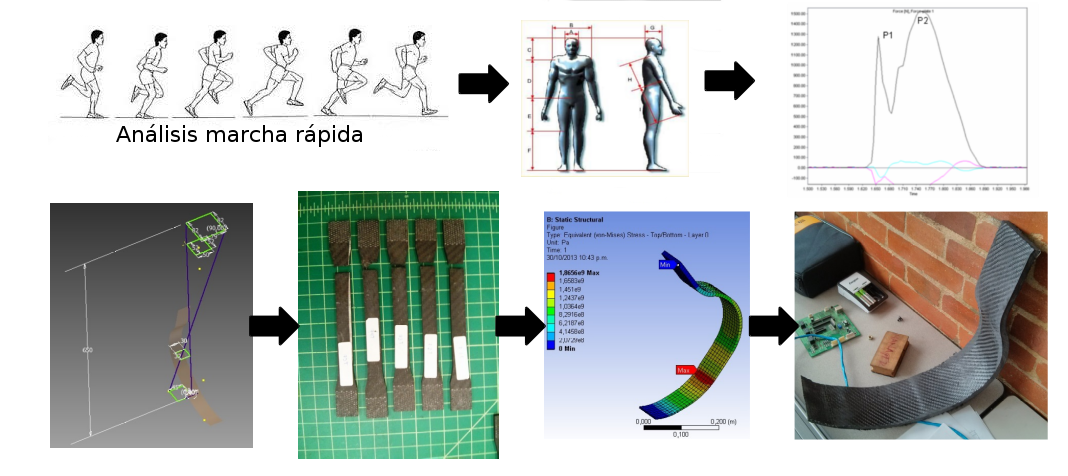
\includegraphics[scale=0.3]{Feathergraphics/tesismaestria}
\par\end{centering}
\caption{Desarrollo tesis de maestría. Imagen realizada por el autor}

\end{figure}

\end{frame}


\begin{frame}{Experiencia previa}

\begin{figure}
\begin{centering}
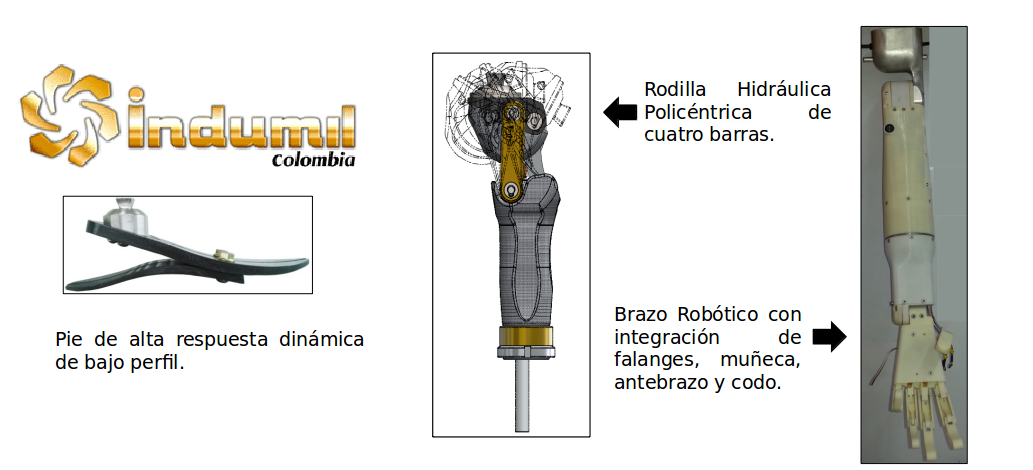
\includegraphics[scale=0.3]{Feathergraphics/experienciaIndumil}
\par\end{centering}
\caption{Experiencia en proyectos relacionados a la temática. Cortesía grupo
DAVINCI e INDUMIL.}

\end{figure}

\end{frame}

\begin{frame}{Diabetes en el mundo}
\begin{columns}[t]


\column{55 mm}
\begin{block}{}
{\footnotesize{}}

\begin{figure}
\begin{centering}
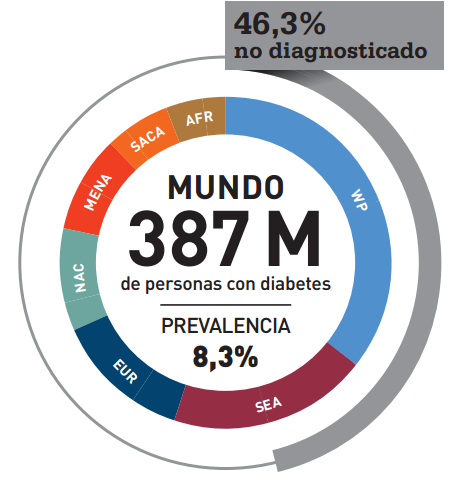
\includegraphics[scale=0.25]{Feathergraphics/proyecciondiabetes}
\par\end{centering}
\caption{Estadísticas de diabetes en el mundo. \cite{ref1}}
\end{figure}
\end{block}

\column{75 mm}

\begin{block}{}
\begin{figure}
\begin{centering}
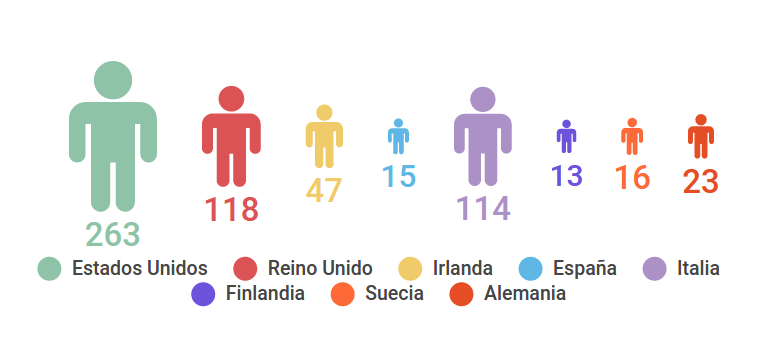
\includegraphics[scale=0.30]{Feathergraphics/ampperyear}
\par\end{centering}
\caption{Número de amputaciones por cada 100.000 habitantes. Adaptado de \cite{KrogerKnut2015} }
\end{figure}

\end{block}
\end{columns}

\end{frame}

\begin{frame}{Diabetes en Colombia}

\begin{columns}[t]


\column{60 mm}

\begin{figure}
\begin{centering}
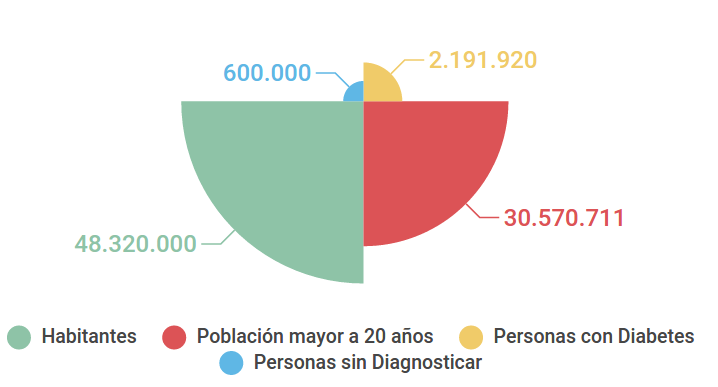
\includegraphics[scale=0.27]{Feathergraphics/DiabetesCol}
\par\end{centering}
\caption{{\scriptsize{}Diabetes en Colombia. Adaptado de \cite{Ramirez2014}. }}

\end{figure}


\column{40 mm}
\begin{exampleblock}{}
{\footnotesize{}}

\begin{itemize}
\item {\footnotesize{}15\% de la población diabética desarrolla una úlcera
de pie, precedente del 85\% de las amputaciones MMII. \cite{Ramirez2014}}{\footnotesize \par}
\item {\footnotesize{}En el estudio de \cite{Pinilla2011} de 307 personas
con diabetes el 1.6\% había sido amputada.}{\footnotesize \par}
\end{itemize}
\end{exampleblock}
\end{columns}

\end{frame}

\begin{frame}{Impacto social en Colombia}

\begin{figure}
\begin{centering}
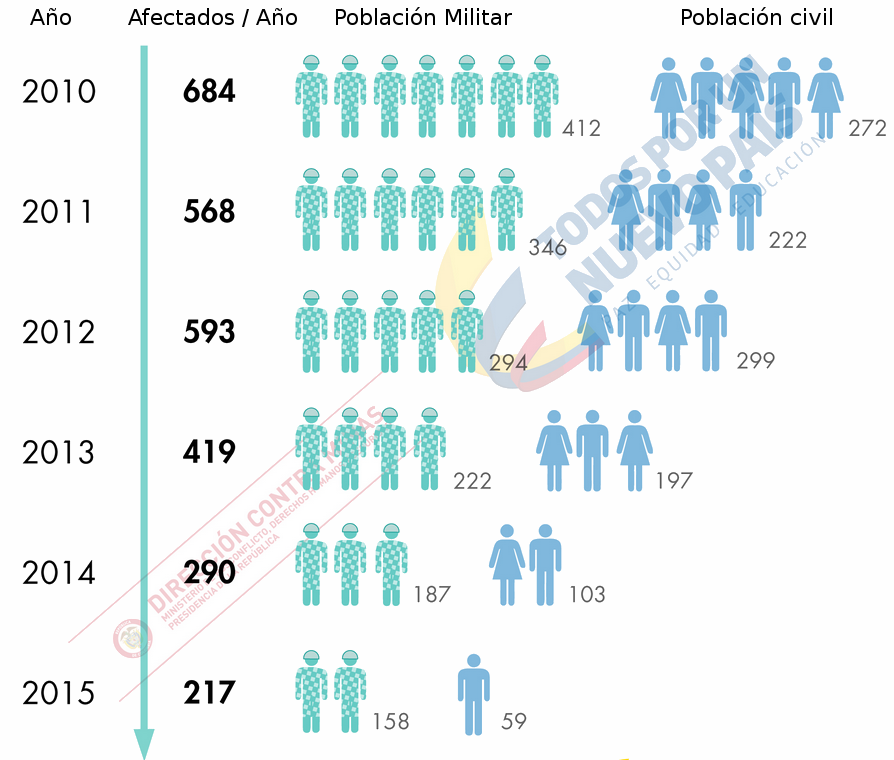
\includegraphics[scale=0.23]{Feathergraphics/DAICMA}
\par\end{centering}
\caption{{\scriptsize{}Situación víctimas MAP y MUSE a diciembre de 2015.\cite{PAICMA}}}
\end{figure}

\end{frame}


\subsection{Avances en prótesis}
\begin{frame}{Investigaciones en el mundo}

\begin{figure}
\begin{centering}
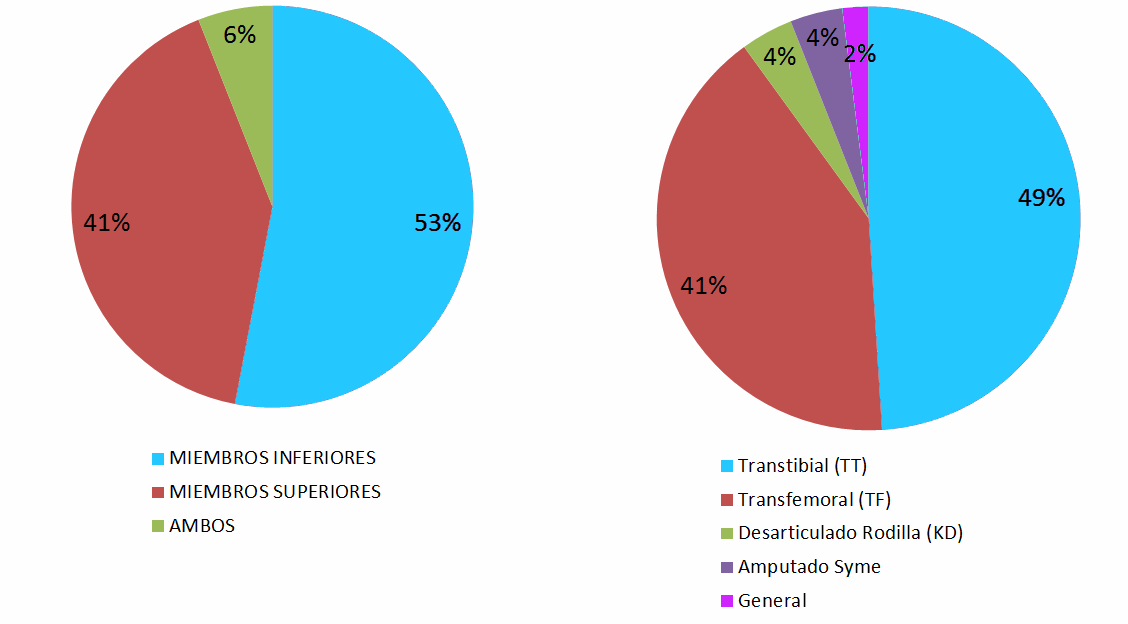
\includegraphics[scale=0.25]{Feathergraphics/Estadisticasestudios}
\par\end{centering}
\caption{Porcentaje de investigaciones en prótesis en los últimos 15 años \cite{Eshraghi2013}.}
\end{figure}
\end{frame}

\begin{frame}{Estado actual prótesis comerciales}

\begin{figure}
\begin{centering}
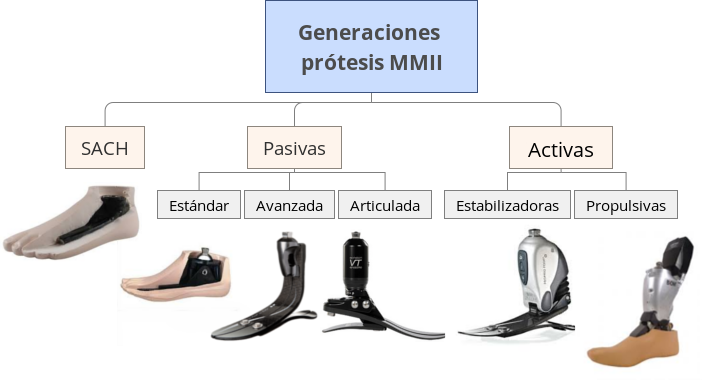
\includegraphics[scale=0.38]{Feathergraphics/Generacionesprotesis}
\par\end{centering}
\caption{{\footnotesize{}Categorización según \cite{Cherelle2014a} de las
prótesis comerciales.} }

\end{figure}

\end{frame}


\section{Estado del arte prótesis pasivas vs biónicas}
\begin{frame}{Histéresis compuestos laminados}

\begin{columns}[t]


\column{70 mm}

\begin{figure}
\begin{centering}
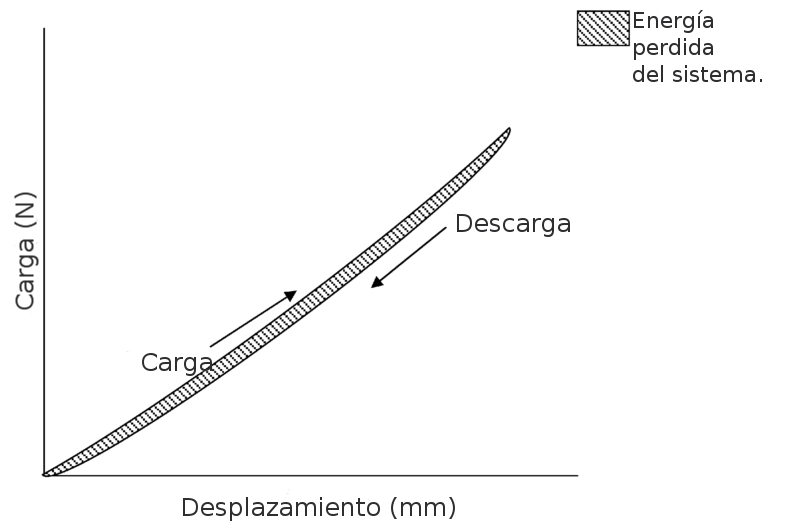
\includegraphics[scale=0.25]{Feathergraphics/hystheresis}
\par\end{centering}
\caption{Histéresis de la fibra de carbono a la compresión. \cite{Nolan2008}}
\end{figure}


\column{50 mm}
\begin{alertblock}{}

\begin{itemize}
\item {\footnotesize{}Buena fuente de trabajo positivo al final de la fase
de apoyo sin requerir baterías \cite{Zelik2014}.}{\footnotesize \par}
\item {\footnotesize{}Sólo reaccionan a la compresión en la etapa de dorsiflexión
\cite{Varol2010}.}{\footnotesize \par}
\item {\footnotesize{}Baja absorción al choque\cite{Au2008}.}{\footnotesize \par}
\end{itemize}
\end{alertblock}
\end{columns}

\end{frame}

\begin{frame}{Patrones asimétricos prótesis ESR}

\begin{alertblock}{}

\begin{itemize}
\item {\scriptsize{}Presentan patrones asimétricos en la marcha \cite{Au2009,Martinez-Villalpando2011,Hill2013a,Bateni2002}.}{\scriptsize \par}
\item {\scriptsize{}Susceptibilidad a la ósteoartritis de rodilla a largo
plazo\cite{Grabowski2013}.}{\scriptsize \par}
\end{itemize}
\begin{figure}
\begin{centering}
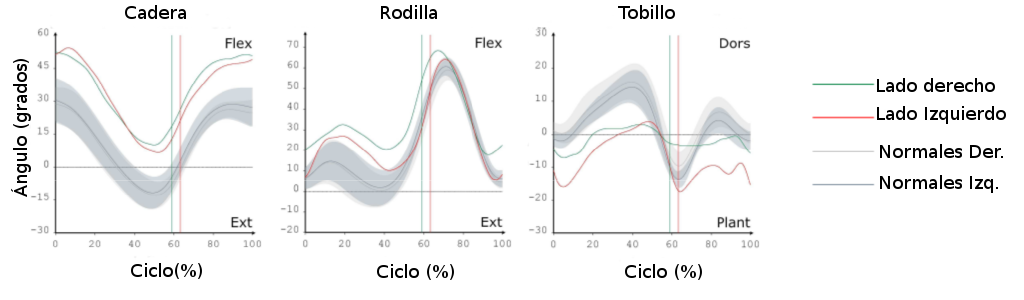
\includegraphics[scale=0.25]{Feathergraphics/Henry}
\par\end{centering}
{\scriptsize{}\caption{Comportamiento cinemático caso clínico UMB}
}{\scriptsize \par}

\end{figure}

\end{alertblock}
\end{frame}

\begin{frame}{Fases de marcha unilateral}

\begin{center}
\begin{figure}
\begin{centering}
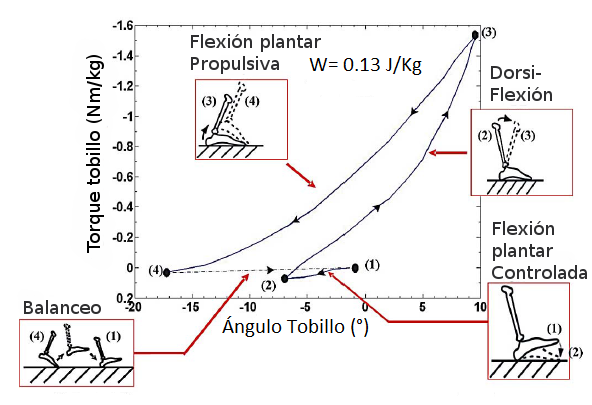
\includegraphics[scale=0.5]{Feathergraphics/cinneticatobillo}
\par\end{centering}
\caption{Comportamiento cinético y cinemático a replicar en el tobillo durante
la fase portante en la marcha normal \cite{Au2009}.}
\end{figure}
\par\end{center}

\end{frame}

\begin{frame}{Biomimetización}

\begin{columns}[t]


\column{65 mm}
\begin{block}{}
{\footnotesize{}}

\begin{figure}
\begin{centering}
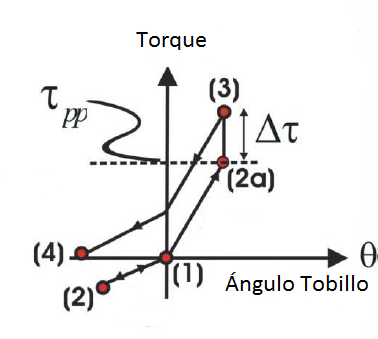
\includegraphics[scale=0.52]{Feathergraphics/cinneticatobillo3}
\par\end{centering}
\caption{{\scriptsize{}Generación del torque faltante en la marcha. \cite{Au2009} }}
\end{figure}

\end{block}

\column{50 mm}
\begin{exampleblock}{}

\begin{itemize}
\item {\footnotesize{}Prótesis ESR: No pueden replicar el trabajo positivo
generado en cada fase de la marcha humana \cite{Esposito2015}.}{\footnotesize \par}
\end{itemize}
\vspace{2 mm}
\begin{itemize}
\item {\footnotesize{}Prótesis Biónicas: requieren una mimetización más
detallada\cite{Hill2013a}.}{\footnotesize \par}
\end{itemize}
\vspace{2 mm}
\begin{itemize}
\item {\footnotesize{}Presenta una trayectoria más estable en comparación
a las pasivas\cite{Hill2013a}.}{\footnotesize \par}
\end{itemize}
\end{exampleblock}
\end{columns}

\end{frame}

\begin{frame}{Consumo metabólico prótesis ESR vs Biónicas}

\begin{columns}[t]


\column{65 mm}
\begin{block}{}
{\footnotesize{}}

\begin{figure}
\begin{centering}
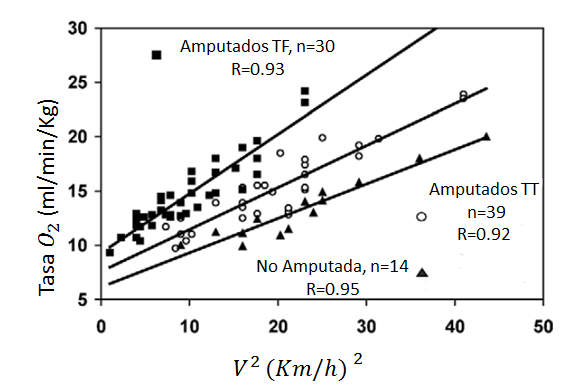
\includegraphics[scale=0.42]{Feathergraphics/consumo}
\par\end{centering}
\caption{{\scriptsize{}Consumo para amputados TFA, TTA y no amputados \cite{Schmalz2002}.}}
\end{figure}

\end{block}

\column{50 mm}
\begin{exampleblock}{}

\begin{itemize}
\item {\scriptsize{}ESR: Reducción velocidad de marcha (30\% a 40\%)\cite{Schmalz2002}.}{\scriptsize \par}
\end{itemize}
\vspace{2 mm}
\begin{itemize}
\item {\scriptsize{}Biónicas: Reducción de la demanda metabólica hasta 16\%
\cite{Herr2010,Esposito2015}.}{\scriptsize \par}
\end{itemize}
\vspace{2 mm}
\begin{itemize}
\item {\scriptsize{}Biónicas: Aumento en la velocidad preferida hasta en
un 10\% en comparación a las ESR\cite{Gates2013}.}{\scriptsize \par}
\end{itemize}
\end{exampleblock}
\end{columns}

\end{frame}

\begin{frame}{Cargas irregulares prótesis ESR vs. Biónicas}

\begin{columns}[t]


\column{60 mm}

\begin{figure}
\begin{centering}
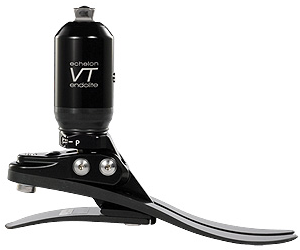
\includegraphics[scale=0.4]{Feathergraphics/echelon}
\par\end{centering}
\caption{Prótesis pasiva con actuador hidráulico.\cite{springking}}
\end{figure}


\column{60 mm}
\begin{exampleblock}{}

\begin{itemize}
\item {\footnotesize{}ESR: crea resistencia a la rotación articular de tobillo
\cite{DeAsha2014}.}{\footnotesize \par}
\item {\footnotesize{}Biónicas: Reducciones en la presión pico en el contacto
de talón en comparación a las prótesis ESR \cite{Hill2013a}.}{\footnotesize \par}
\item {\footnotesize{}Biónicas: Decrecimientos en la fuerza resultante pico
y en los momentos aductores de rodilla del lado inafectado \cite{Grabowski2013}.}{\footnotesize \par}
\end{itemize}
\end{exampleblock}
\end{columns}

\end{frame}

\begin{frame}{Debilidades prótesis activas}

\begin{columns}[t]


\column{60 mm}
\begin{alertblock}{}

\begin{itemize}
\item {\scriptsize{}Causan altos niveles de ruido \cite{boston}.}{\scriptsize \par}
\item {\scriptsize{}No es escalable \cite{BIOMASME}.}{\scriptsize \par}
\item {\scriptsize{}No cumplen con el concepto de antropomorficidad\cite{BIOMASME}.}{\scriptsize \par}
\end{itemize}
\end{alertblock}
\begin{exampleblock}{}

\begin{itemize}
\item {\footnotesize{}El sistema reemplaza la pérdida muscular y tendinosa\cite{Varol2010}. }{\footnotesize \par}
\item {\footnotesize{}Reconoce diferentes terrenos y velocidades \cite{Lawson2011}. }{\footnotesize \par}
\item {\footnotesize{}Produce potencia positiva mecánica\cite{Martinez-Villalpando2009}.}{\footnotesize \par}
\end{itemize}
\end{exampleblock}

\column{60 mm}

\begin{figure}
\begin{centering}
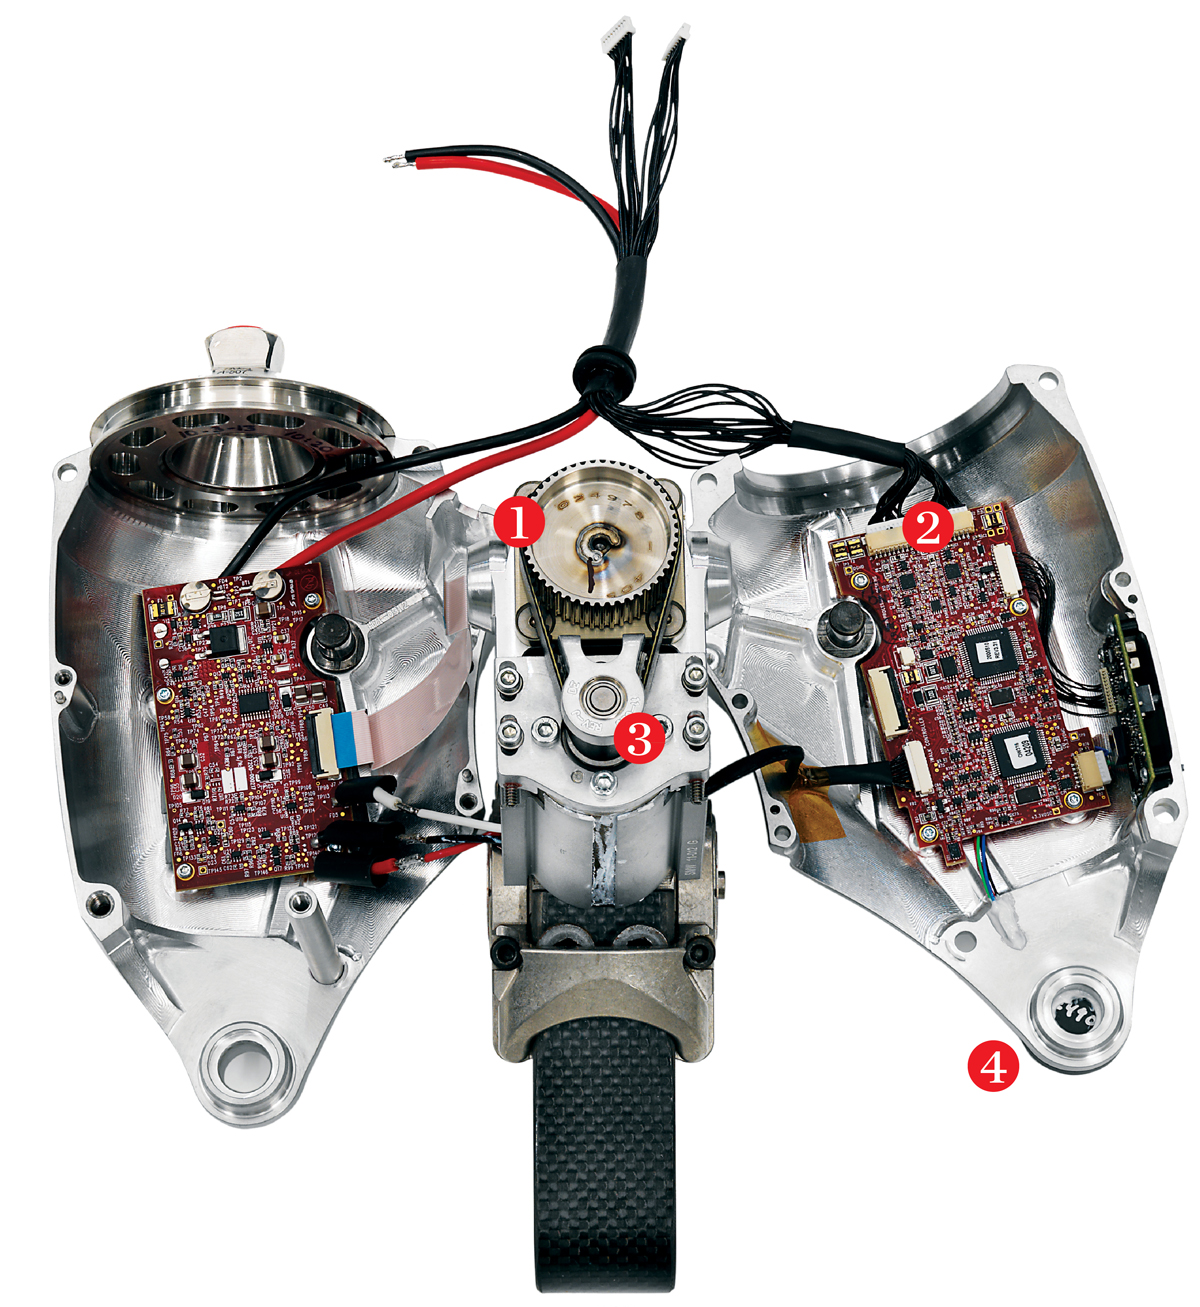
\includegraphics[scale=0.11]{Feathergraphics/Bionaked}
\par\end{centering}
{\scriptsize{}\caption{Configuración interna Biom \cite{boston}}
}{\scriptsize \par}

\end{figure}

\end{columns}

\end{frame}

\begin{frame}{Costos}

\begin{block}{Prótesis ESR son Económicas en relación a las activas}
\end{block}
\begin{figure}
\begin{centering}
\begin{tabular}{|c|c|c|c|}
\hline 
\multicolumn{2}{|c|}{Prótesis Pasivas} & \multicolumn{2}{c|}{Prótesis Biónicas}\tabularnewline
\hline 
\hline 
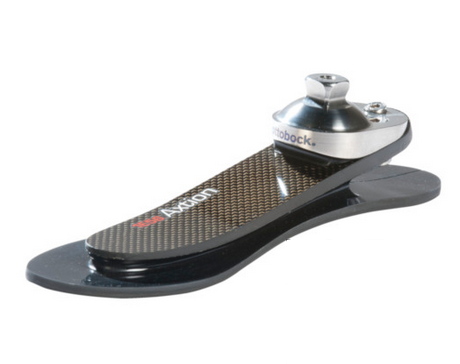
\includegraphics[scale=0.15]{Feathergraphics/axtion} & 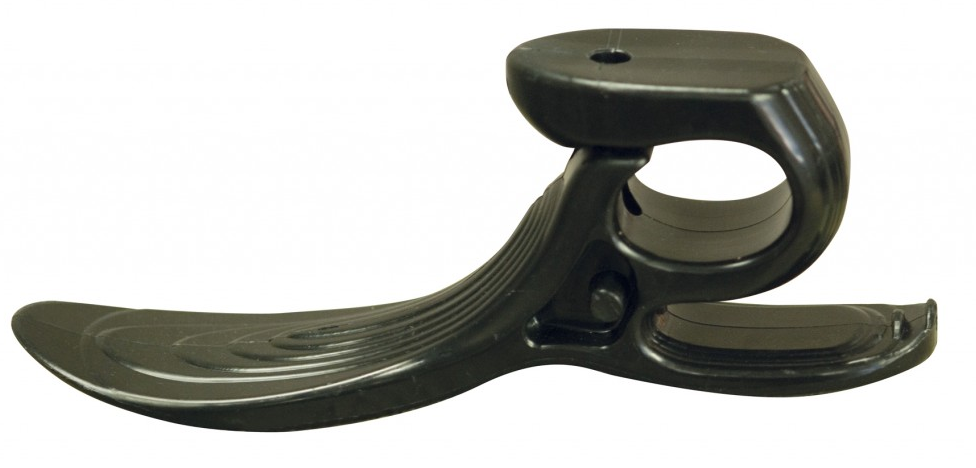
\includegraphics[scale=0.1]{Feathergraphics/niagara} & 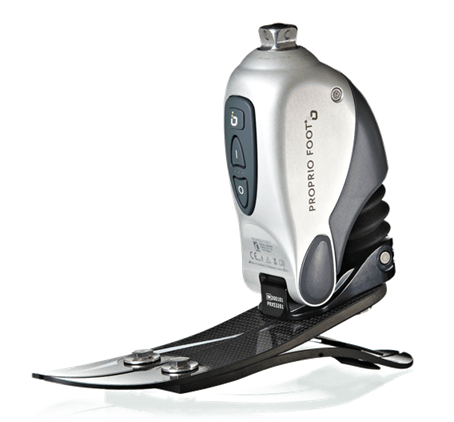
\includegraphics[scale=0.15]{Feathergraphics/proprio} & 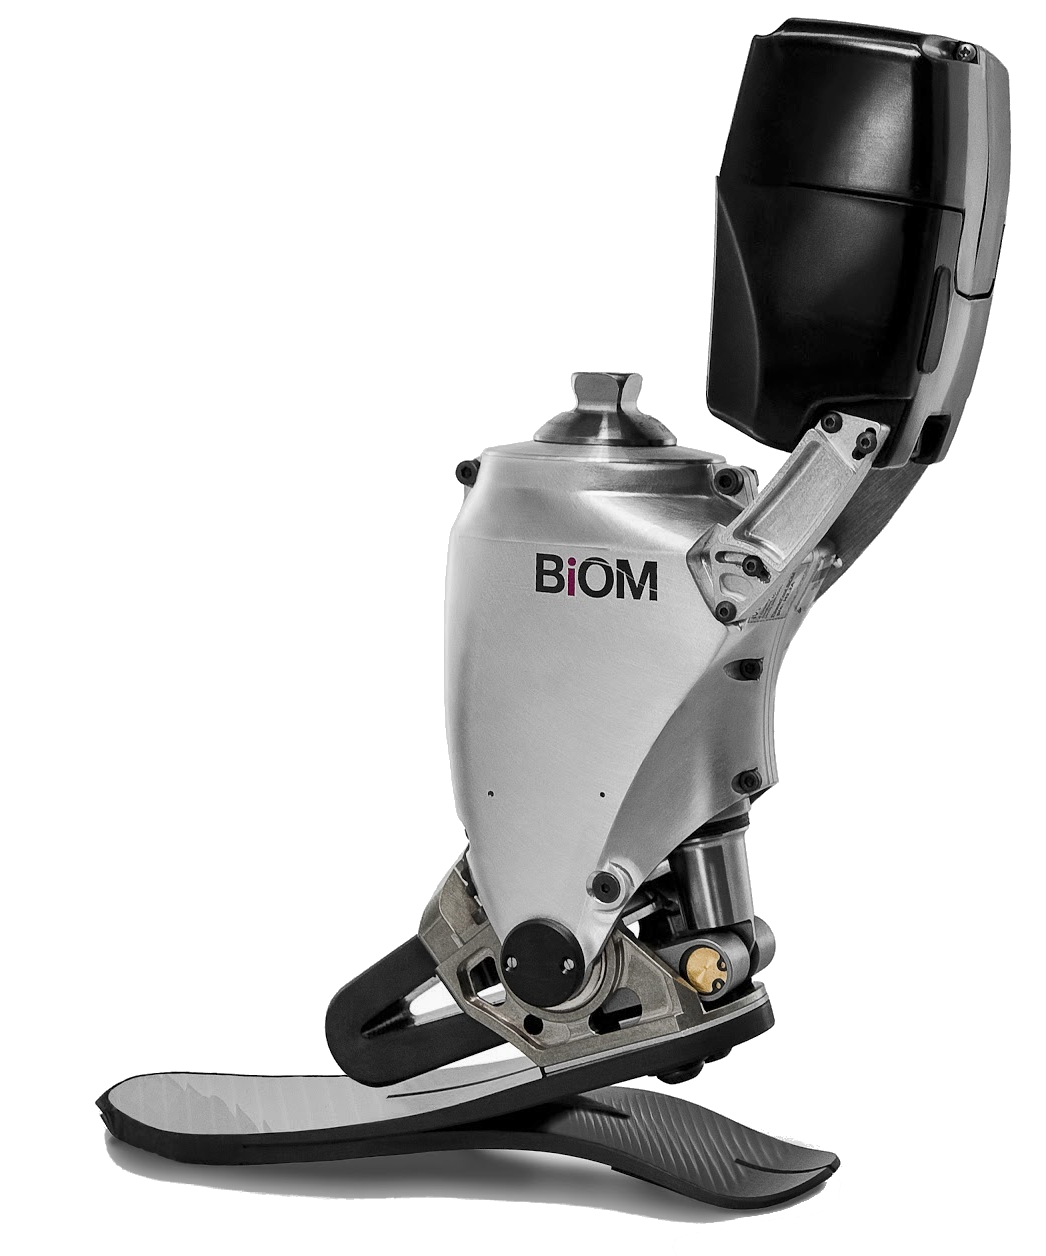
\includegraphics[scale=0.05]{Feathergraphics/BiOM}\tabularnewline
\hline 
{\footnotesize{}COP\$3.000.000} & {\footnotesize{}U\$ 35\cite{Niagara}} & {\footnotesize{}U\$ 25.000 \cite{bloomberg}} & {\footnotesize{}U\$ 40.000 \cite{boston}}\tabularnewline
\hline 
\end{tabular}
\par\end{centering}
\caption{De Izq. a Der.: Axtion foot de OttoBock$\circledR$, Niagara foot,
Proprio Ossur$\circledR$ y Biom de Bionx$\circledR$. Imágenes obtenidas
de las páginas oficiales.}
\end{figure}

\end{frame}

\begin{frame}{Resumen comparativo}

\begin{table}
\begin{centering}
\begin{tabular}{|>{\centering}p{24mm}|>{\centering}p{45mm}|>{\centering}p{24mm}|}
\hline 
{\footnotesize{}Prótesis ESR} & {\footnotesize{}Aspecto} & {\footnotesize{}Prótesis Biónicas}\tabularnewline
\hline 
\hline 
{\footnotesize{}-25\%} & {\footnotesize{}Costo metabólico} & {\footnotesize{}-10\%}\tabularnewline
\hline 
{\footnotesize{}-30\%} & {\footnotesize{}Velocidad preferida} & {\footnotesize{}-20\%}\tabularnewline
\hline 
{\footnotesize{}Hasta 84 \%} & {\footnotesize{}Trabajo positivo} & {\footnotesize{}35 J}\tabularnewline
\hline 
{\footnotesize{}Mejores al SACH} & {\footnotesize{}Parámetros temporales} & {\footnotesize{}Mejores a las ESR}\tabularnewline
\hline 
{\footnotesize{}Fuera de rango} & {\footnotesize{}Parámetros cinemáticos y cinéticos} & {\footnotesize{}Mejores a las ESR}\tabularnewline
\hline 
{\footnotesize{}Si} & {\footnotesize{}Antropométricas} & {\footnotesize{}No todas}\tabularnewline
\hline 
{\footnotesize{}Indefinida} & {\footnotesize{}Autonomía} & {\footnotesize{}Limitada}\tabularnewline
\hline 
{\footnotesize{}Mayor} & {\footnotesize{}Presión contacto} & {\footnotesize{}Menor}\tabularnewline
\hline 
{\footnotesize{}Menor} & {\footnotesize{}Estabilidad} & {\footnotesize{}Mayor}\tabularnewline
\hline 
{\footnotesize{}Accesible} & {\footnotesize{}Precio} & {\footnotesize{}Muy alto}\tabularnewline
\hline 
\end{tabular}
\par\end{centering}
\caption{Resumen comparativo prótesis ESR vs Biónicas}

\end{table}

\end{frame}

\begin{frame}{Estado actual actuadores protésicos}

\begin{tabular}{|>{\centering}p{20mm}|>{\centering}p{30mm}|>{\centering}p{45mm}|}
\hline 
\textbf{\scriptsize{}Tipo} & \textbf{\scriptsize{}Representación gráfica} & \textbf{\scriptsize{}Implementado en}\tabularnewline
\hline 
\hline 
{\scriptsize{}Actuador rígido} & {\scriptsize{}\vspace{1 mm}}{\scriptsize \par}

{\scriptsize{}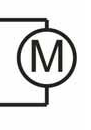
\includegraphics[scale=0.4]{Feathergraphics/DD}} & {\scriptsize{}Proprio Ossur $\circledR$}\tabularnewline
\hline 
{\scriptsize{}Actuador Elástico en Serie (SEA)} & {\scriptsize{}\vspace{1 mm}}{\scriptsize \par}

{\scriptsize{}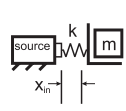
\includegraphics[scale=0.6]{Feathergraphics/SEAmodel}} & {\scriptsize{}-SPARKy (Spring Ankle with Regenerative Kinetics) \cite{Holgate2008,Bellman2008}.}{\scriptsize \par}

{\scriptsize{}-Prototipo transfemoral de la U. Vanderbilt.\cite{Sup2008,Sup2009}}\tabularnewline
\hline 
{\scriptsize{}SEA con Embrague (CSEA)} & {\scriptsize{}\vspace{1 mm}}{\scriptsize \par}

{\scriptsize{}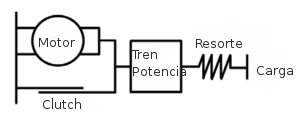
\includegraphics[scale=0.35]{Feathergraphics/CSEA}} & {\scriptsize{}Prototipo de rodilla de iWalk$\circledR$.}\tabularnewline
\hline 
\end{tabular}
\end{frame}

\begin{frame}{Estado actual actuadores protésicos}

\begin{tabular}{|>{\centering}p{20mm}|>{\centering}p{45mm}|>{\centering}p{35mm}|}
\hline 
\textbf{\small{}Tipo} & \textbf{\small{}Representación gráfica} & \textbf{\small{}Implementado en}\tabularnewline
\hline 
{\small{}SEA con transmisión continua variable} & {\small{}\vspace{1 mm}}{\small \par}

{\small{}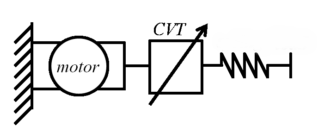
\includegraphics[scale=0.35]{Feathergraphics/CVSEA}} & {\small{}No implementado a la fecha.}\tabularnewline
\hline 
{\small{}SEA con elasticidad en paralelo} & {\small{}\vspace{1 mm}}{\small \par}

{\small{}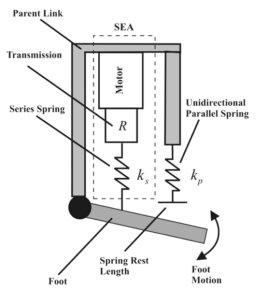
\includegraphics[scale=0.35]{Feathergraphics/BiOMmodel}} & {\small{}Pie BiOM de iWalk $\circledR.$\cite{herr2011controlling,herr2014powered,han2012controlling,han2014controlling}}\tabularnewline
\hline 
\end{tabular}
\end{frame}

\begin{frame}{Estado actual actuadores protésicos}

\begin{tabular}{|>{\centering}p{20mm}|>{\centering}p{40mm}|>{\centering}p{30mm}|}
\hline 
\textbf{\footnotesize{}Tipo } & \textbf{\footnotesize{}Representación gráfica} & \textbf{\footnotesize{}Implementado en}\tabularnewline
\hline 
\hline 
{\footnotesize{}Actuador elástico con amortiguador en serie (SEDA)} & {\footnotesize{}\vspace{1 mm}}{\footnotesize \par}

{\footnotesize{}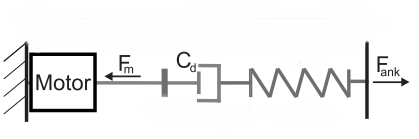
\includegraphics[scale=0.3]{Feathergraphics/SEDA}} & {\footnotesize{}No implementado \cite{Eslamy2013}.}\tabularnewline
\hline 
{\footnotesize{}Actuador elástico con amortiguador en paralelo (PEDA)} & {\footnotesize{}\vspace{1 mm}}{\footnotesize \par}

{\footnotesize{}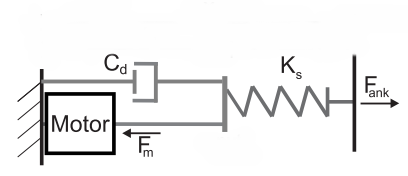
\includegraphics[scale=0.3]{Feathergraphics/PEDA}} & {\footnotesize{}No implementado \cite{Eslamy2013}.}\tabularnewline
\hline 
{\footnotesize{}Actuador de Rigidez Variable} & {\footnotesize{}\vspace{1 mm}}{\footnotesize \par}

{\footnotesize{}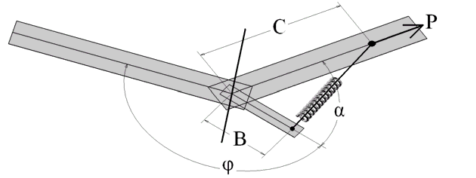
\includegraphics[scale=0.25]{Feathergraphics/maccepa2}} & {\footnotesize{}Proyecto CYBERLEG. \cite{Cherelle2014}}\tabularnewline
\hline 
\end{tabular}
\end{frame}


\section{Identificación del problema}

\subsection{Estrategias de generación de energía}
\begin{frame}{Estrategias de Generación}

\begin{figure}
\begin{centering}
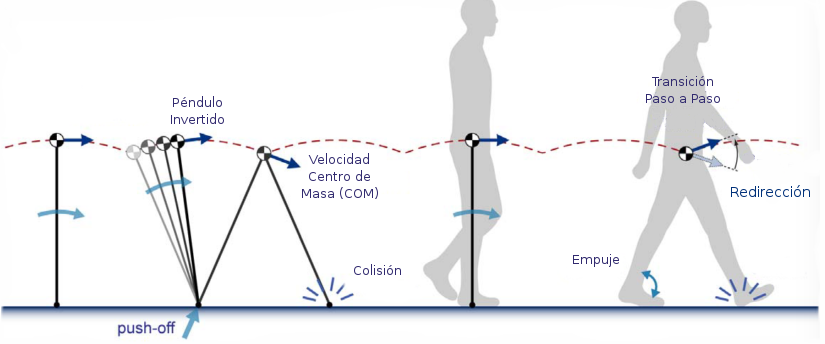
\includegraphics[scale=0.35]{Feathergraphics/transicion}
\par\end{centering}
{\scriptsize{}\caption{{\scriptsize{}Reciclaje de energía perdida en la marcha}.\cite{Collins2010}}
}{\scriptsize \par}
\end{figure}
\end{frame}

\begin{frame}{Estrategias de Generación}

\begin{figure}
\begin{centering}
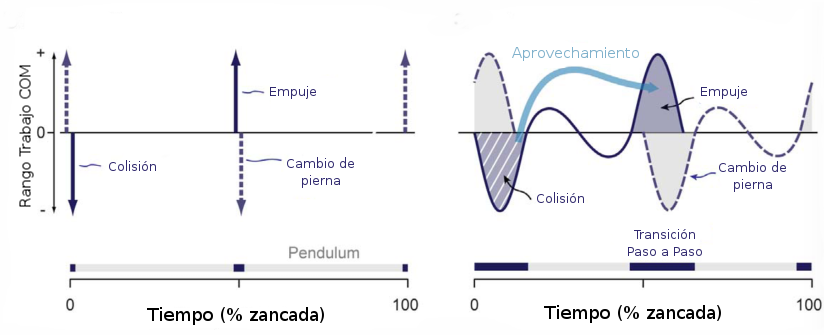
\includegraphics[scale=0.35]{Feathergraphics/transicion2}
\par\end{centering}
{\scriptsize{}\caption{{\scriptsize{}Transición de la energía perdida en la marcha.\cite{Collins2010}}}
}{\scriptsize \par}
\end{figure}
\end{frame}


\subsection{Problemática actual}
\begin{frame}{Demanda Energética}

\begin{figure}
\begin{centering}
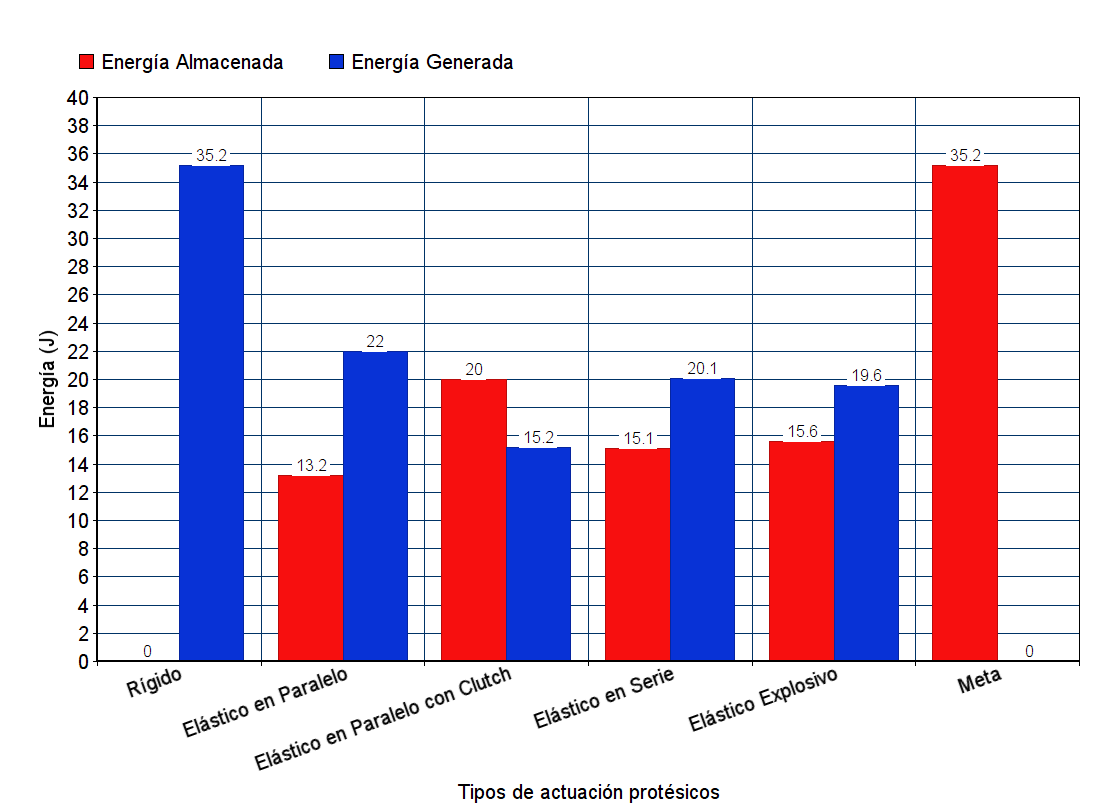
\includegraphics[scale=0.31]{Feathergraphics/20160310072328}
\par\end{centering}
{\tiny{}\caption{{\scriptsize{}Energía almacenada vs Energía generada \cite{Cherelle2014a}.}}
}{\tiny \par}

\end{figure}

\end{frame}

\begin{frame}{Torque, velocidad y potencia}

\begin{figure}
\begin{centering}
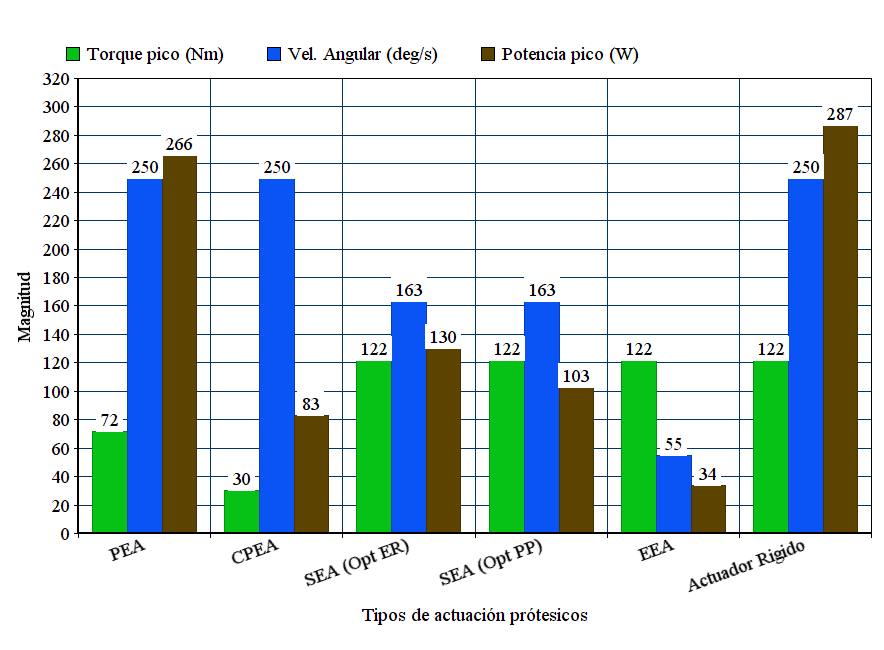
\includegraphics[scale=0.28]{Feathergraphics/20160113110039}
\par\end{centering}
{\tiny{}\caption{{\tiny{}Variables mecánicas actuadores protésicos \cite{Cherelle2014a}}.}
}{\tiny \par}

\end{figure}

\end{frame}

\begin{frame}{Relación problemática}

\begin{figure}
\begin{centering}
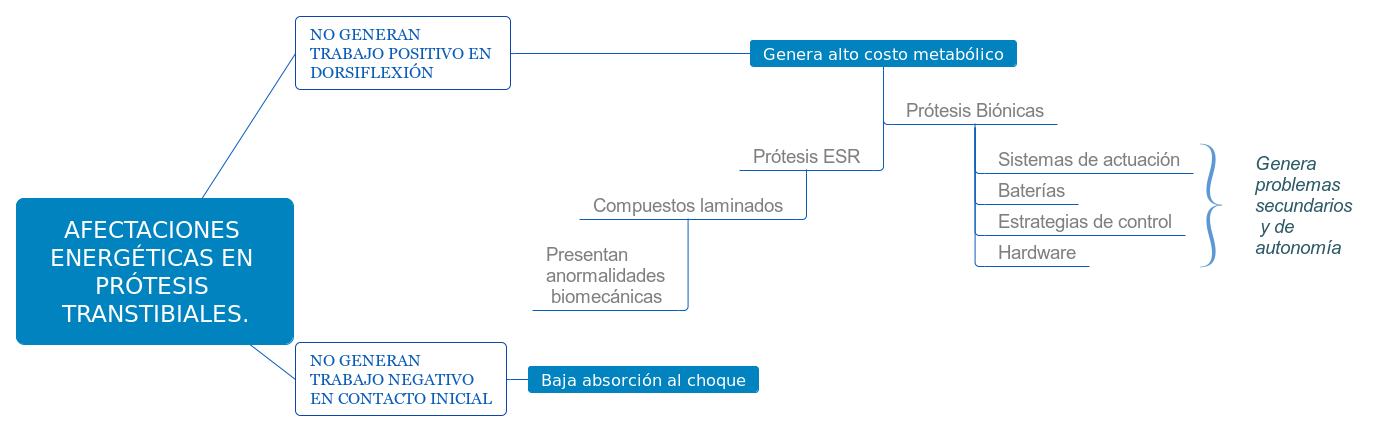
\includegraphics[scale=0.24]{Feathergraphics/Afectaciones_energeticas_en_protesis_transtibiales.png}
\par\end{centering}
\caption{Mapa conceptual problemática}

\end{figure}

\end{frame}

\begin{frame}{Identificación del problema}

\begin{exampleblock}{Problemática actual}

\begin{itemize}
\item Las prótesis pasivas actuales para amputaciones transtibiales, provocan
alteraciones en los parámetros dinámicos de la marcha normal para
el amputado, a causa de ausencia de trabajo positivo.
\end{itemize}
\end{exampleblock}
\end{frame}


\subsection{Pregunta de investigación}
\begin{frame}{Identificación del problema}

\begin{block}{Pregunta de investigación}

¿Qué configuración de prótesis transtibial basada en la dinámica pasiva,
generará el trabajo positivo en la fase de apoyo final a través del
aprovechamiento de la energía perdida en la colisión del contacto
inicial de la marcha humana, hasta reducir las alteraciones dinámicas
presentes en usuarios con prótesis pasivas?

\end{block}
\end{frame}

\begin{frame}{Identificación del problema}

\begin{block}{Hipótesis}

Una prótesis transtibial configurada para aprovechar la energía perdida
del contacto inicial de la marcha, permitirá generar el trabajo positivo
necesario en la fase de apoyo final, sin necesidad de recurrir a sistemas
de actuación activos. 

\end{block}
\end{frame}


\section{Objetivos}

\subsection{Objetivo General}
\begin{frame}{Objetivos}

\begin{alertblock}{Objetivo General}

Proponer una configuración de prótesis transtibial, que genere a través
de un sistema dinámico pasivo el trabajo positivo necesario en la
dorsiflexión máxima, aprovechando la energía perdida en el contacto
inicial de la marcha.
\end{alertblock}
\end{frame}


\subsection{Objetivos Específicos}
\begin{frame}{Objetivos}

\begin{exampleblock}{Objetivos específicos}

\begin{enumerate}
\item Identificar los parámetros biomecánicos y el diagrama del ciclo de
trabajo a un usuario de prótesis pasiva con amputación unilateral
transtibial para determinar los requerimientos energéticos.
\item Obtener el modelo dinámico de la prótesis transtibial que aproveche
la energía durante el contacto inicial y el apoyo medio para entregarla
en la fase de apoyo final de la marcha mediante la aplicación de sólidos
celulares en manufactura aditiva.
\item Validar la configuración protésica transtibial generada, en comparación
a un modelo protésico pasivo.
\end{enumerate}
\end{exampleblock}
\end{frame}


\section{Metodología y actividades}
\begin{frame}{Fases}

\begin{figure}
\centering{}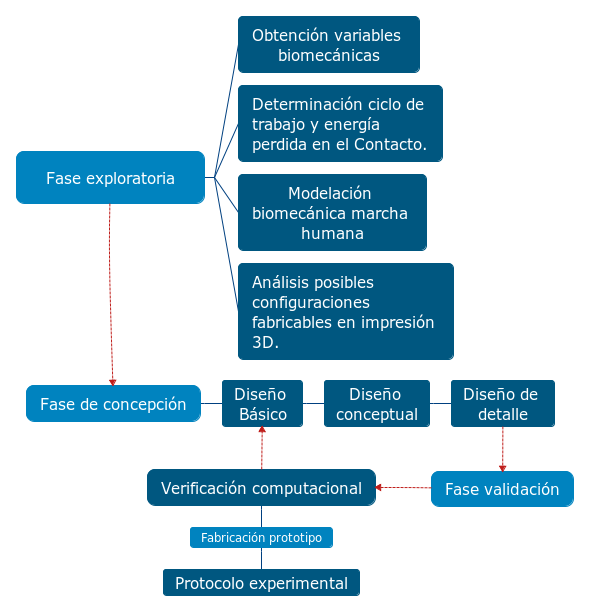
\includegraphics[scale=0.35]{Feathergraphics/Fase_exploratoria}
\end{figure}

\end{frame}

\begin{frame}{Fase exploratoria}

\begin{block}{{\scriptsize{}Recopilar y/o adquirir los principales comportamientos
biomecánicos mencionados por \cite{Sagawa2011} de la marcha estándar
con amputación transtibial para realizar la modelación biomecánica
en Opensim$\circledR$ a un usuario de prótesis ESR y a otro sujeto
sin patologías.}}
\end{block}
\noindent \begin{center}
\begin{tabular}{|>{\raggedright}m{20mm}|>{\centering}p{25mm}|>{\centering}p{25mm}|}
\hline 
\multicolumn{3}{|c|}{{\tiny{} \textbf{Parámetros Biomecánicos}}}\tabularnewline
\hline 
{\tiny{} \textbf{Parámetros Espacio-temporales}} & {\tiny{} \textbf{Ángulos articulares}} & {\tiny{} \textbf{Potencia Articular}}\tabularnewline
\hline 
\hline 
\multirow{5}{20mm}{{\tiny{}Velocidad, cadencia, t. ciclo, t. fase apoyo, t. fase balanceo,
t. soporte simple...}} & {\tiny{}Ángulos de cadera, Rodilla y Tobillo} & {\tiny{}Cadera, Rodilla y Tobillo}\tabularnewline
\cline{2-3} 
 & {\tiny{}\textbf{Momentos articulares}} & {\tiny{}\textbf{Plataforma}}\tabularnewline
\cline{2-3} 
 & \multirow{3}{25mm}{{\tiny{}Cadera, Rodilla y Tobillo}} & \multirow{3}{25mm}{{\tiny{}Fuerza de Reacción anteroposterior, vertical y anteroposterior}}\tabularnewline
 &  & \tabularnewline
 &  & \tabularnewline
\hline 
\end{tabular}
\par\end{center}

\end{frame}

\begin{frame}{Actividades objetivo 1}

\begin{columns}[t]


\column{28 mm}
\begin{block}{}

\begin{itemize}
\item {\scriptsize{}Realizar solicitud comité de ética en UN y UMB.}{\scriptsize \par}
\end{itemize}
\end{block}

\column{40 mm}
\begin{block}{}

\begin{itemize}
\item {\scriptsize{}Realizar protocolo adquisición de datos experimentales
en laboratorio de marcha.}{\scriptsize \par}
\item {\scriptsize{}Paciente sin patologías y paciente con amputación transtibial.}{\scriptsize \par}
\item {\scriptsize{}Tomar fotos con marcadores.}{\scriptsize \par}
\end{itemize}
\end{block}

\column{25 mm}
\begin{block}{}

\begin{itemize}
\item {\scriptsize{}Adaptar el modelo biomecánico}{\scriptsize \par}
\item {\scriptsize{}Obtener la magnitud de energía perdida}{\scriptsize \par}
\end{itemize}
\end{block}

\column{30 mm}
\begin{block}{}

\begin{itemize}
\item {\scriptsize{}Verificación computacional con estudios reales.}{\scriptsize \par}
\end{itemize}
\end{block}
\end{columns}

\end{frame}

\begin{frame}{Proceso de Opensim}

\begin{block}{Reconstruir mediante modelos computacionales la dinámica de marcha
estándar con alteraciones patológicas.}
\end{block}
\begin{center}
\begin{figure}
\begin{centering}
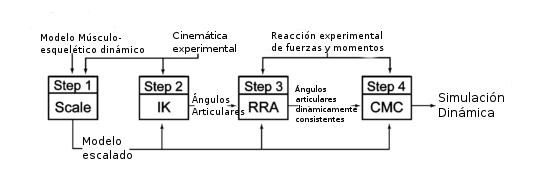
\includegraphics[scale=0.55]{Feathergraphics/muscle-driven-sim}
\par\end{centering}
\caption{Proceso de modelación de la marcha en Opensim}

\end{figure}
\par\end{center}

\end{frame}

\begin{frame}{Metodología fase de concepción}

\begin{columns}[t]


\column{60 mm}

{\footnotesize{}A través de herramientas para simulación de sistemas
dinámicos, realizar el diseño y simulación del modelo siguiendo la
metodología propuesta por \cite{Hicks2014}.}{\footnotesize \par}

\column{60 mm}

\begin{figure}
\begin{centering}
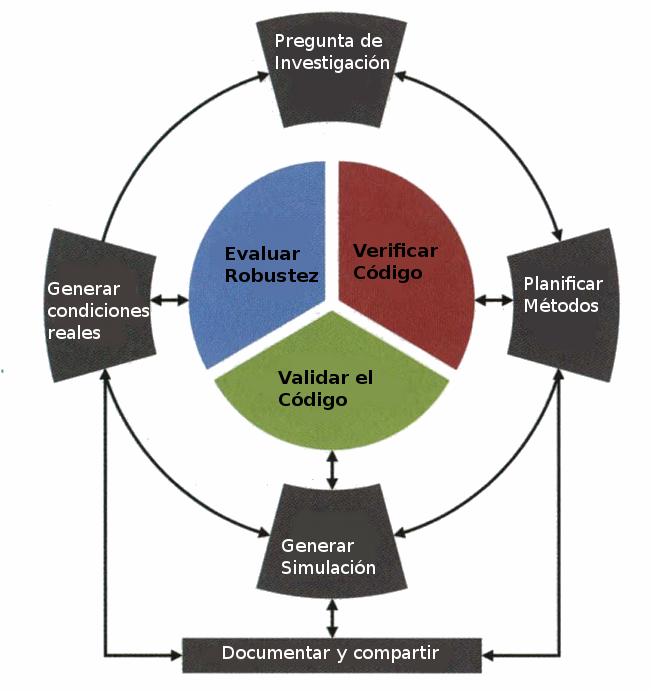
\includegraphics[scale=0.3]{Feathergraphics/verificationprocess}
\par\end{centering}
\caption{{\tiny{}Proceso validación y verificación modelos \cite{Hicks2014}.}}
\end{figure}

\end{columns}

\end{frame}

\begin{frame}{Actividades objetivo No. 2}

\begin{block}{}

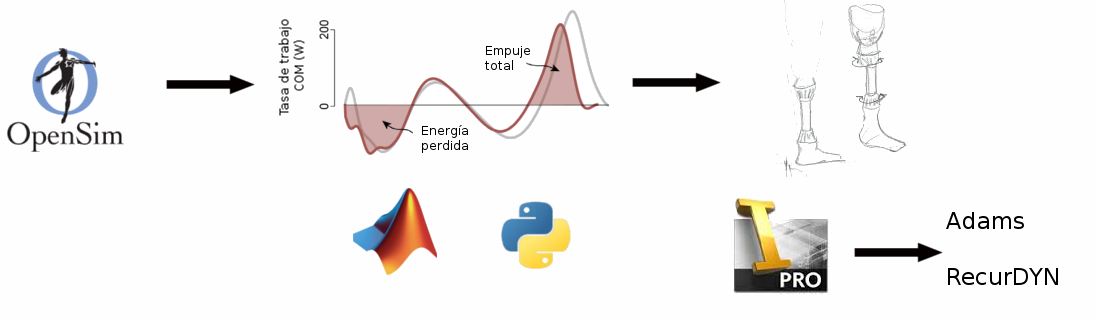
\includegraphics[scale=0.28]{Feathergraphics/Actividades2}
\end{block}
\end{frame}

\begin{frame}{Actividades objetivo No. 2}

\begin{block}{Actividades}

\begin{enumerate}
\item {\scriptsize{}Determinar de manera analítica el ciclo de trabajo interno
y externo de los modelos obtenidos con una herramienta científica
personalizada como Python$\circledR$ o Matlab$\circledR$.}{\scriptsize \par}
\item {\scriptsize{}Determinar las propiedades mecánicas específicas de
cada sección de la configuración de acuerdo a los parámetros biomecánicos
obtenidos anteriormente.}{\scriptsize \par}
\item {\scriptsize{}Determinar la configuración del material celular tal
que cumpla con las condiciones necesarias para la acumulación energética
y así garantizar la fabricación mediante técnicas de manufactura aditiva.}{\scriptsize \par}
\item {\scriptsize{}Verificar el modelo de absorción de energía y plasmarlo
en software de simulación dinámica combinado con elementos finitos,
bien sea en software como AutoDYN$\circledR$, ABAQUS$\circledR$
o Elmer$\circledR$.}{\scriptsize \par}
\item {\scriptsize{}De los parámetros mecánicos expuestos en la norma ISO
22675, evaluar la resistencia mecánica necesaria del modelo protésico.}{\scriptsize \par}
\item {\scriptsize{}Obtener el ciclo de trabajo de la nueva configuración
de acuerdo a los parámetros biomecánicos del modelo de amputación
transtibial.}{\scriptsize \par}
\item {\scriptsize{}Realizar el proceso de verificación y validación estructural
del modelo mediante técnicas }\emph{\scriptsize{}in silico}{\scriptsize{}.}{\scriptsize \par}
\end{enumerate}
\end{block}
\end{frame}

\begin{frame}{Metodología objetivo No. 3}

\begin{columns}[t]


\column{30 mm}
\begin{block}{{\footnotesize{}Validar la configuración protésica transtibial generada,
en comparación a un modelo protésico pasivo.}}

{\footnotesize{}Realizar la impresión 3D del modelo generado y validar
el trabajo positivo generado en el nuevo concepto mediante pruebas
de marcha en dos o más usuarios con amputación unilateral transtibial.}{\footnotesize \par}
\end{block}

\column{90 mm}

\begin{figure}
\begin{centering}
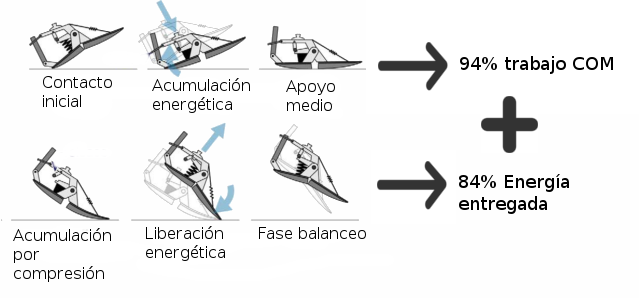
\includegraphics[scale=0.4]{Feathergraphics/Actividades3}
\par\end{centering}
\caption{{\scriptsize{}Secuencia de absorción energética en fases de marcha.
Adaptado de \cite{Collins2010}}}
\end{figure}

\end{columns}

\end{frame}

\begin{frame}{Actividades objetivo No. 3}

\begin{enumerate}
\item Solicitar nuevamente el aval del comité de ética a las entidades respectivas.
\item Realizar la comparación del trabajo positivo generado durante la transición
paso a paso de los tres casos de referencia (patológico con ESR, patológico
con el nuevo concepto y no patológico)
\item Evaluar las diferencias significativas en cada instancia de la marcha
y emitir conclusiones.
\end{enumerate}
\end{frame}

\begin{frame}{Metodología objetivo No. 4}

\begin{columns}[t]


\column{65 mm}
\begin{block}{}

{\scriptsize{}Obtenidos los modelos se procede a la comparación In
silico del nuevo concepto vs. prótesis ESR vs estudios prótesis biónicas.}{\scriptsize \par}

\begin{figure}
\begin{centering}
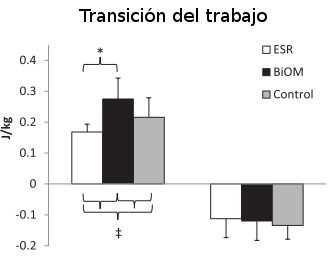
\includegraphics[scale=0.35]{Feathergraphics/Biomvscontrol}
\par\end{centering}
\caption{Estudio comparativo transición del trabajo de BiOM vs Control vs ESR
\cite{Esposito2015}.}

\end{figure}
\end{block}

\column{60 mm}

\begin{figure}
\begin{centering}
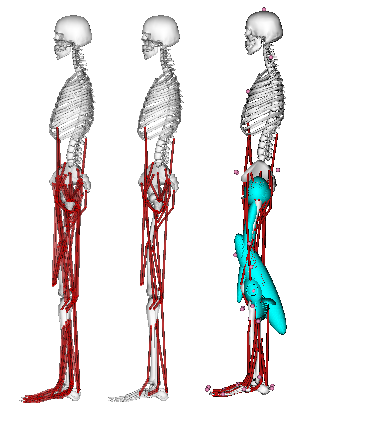
\includegraphics[scale=0.4]{Feathergraphics/2354_2392_SIMM}
\par\end{centering}
\caption{Diferentes modelos músculo-esqueléticos de Opensim. Tomado de Opensim}
\end{figure}

\end{columns}

\end{frame}

\begin{frame}{Metodología objetivo No. 5}

\begin{columns}[t]


\column{50 mm}
\begin{exampleblock}{}

\begin{itemize}
\item {\footnotesize{}Evaluar las capacidades de la tecnología en Manufactura
Aditiva para fabricar el modelo de acuerdo a los parámetros de diseño.}{\footnotesize \par}
\item {\footnotesize{}Realizar pruebas de deformación y respuesta del modelo
con sistemas de visión artificial.}{\footnotesize \par}
\end{itemize}
\end{exampleblock}

\column{60 mm}

\begin{figure}
\begin{centering}
{\scriptsize{}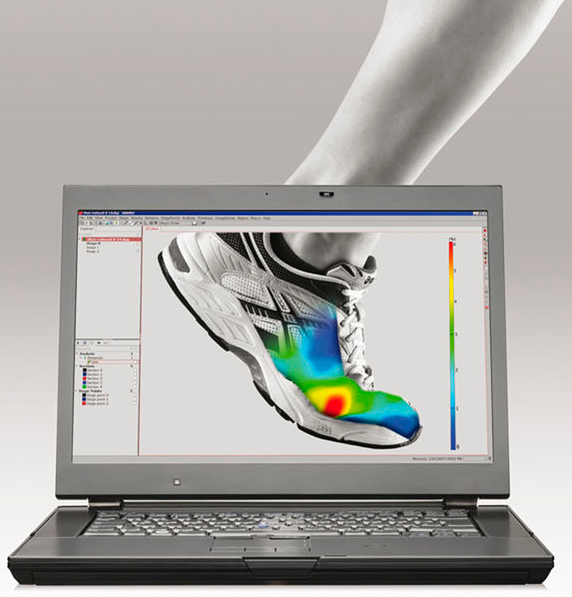
\includegraphics[scale=0.23]{Feathergraphics/strainshoe}}
\par\end{centering}{\scriptsize \par}
\caption{{\scriptsize{}Pruebas de deformación en zapatilla a través de sistemas
de visión artificial. Tomado de www.gom.com.}}
\end{figure}

\end{columns}

\end{frame}


\section{Cronograma y presupuesto}
\begin{frame}{Cronograma}

\begin{table}[H]
\noindent \centering{}%
\begin{tabular}{|>{\centering}p{30mm}|>{\centering}p{2mm}|>{\centering}p{2mm}|>{\centering}p{2mm}|>{\centering}p{2mm}|>{\centering}p{2mm}|>{\centering}p{2mm}|>{\centering}p{2mm}|>{\centering}p{2mm}|>{\centering}p{2mm}|>{\centering}p{3mm}|>{\centering}p{3mm}|>{\centering}p{3mm}|}
\hline 
{\tiny{}\textbf{Tiempo (2 meses)}} & {\tiny{}1} & {\tiny{}2} & {\tiny{}3} & {\tiny{}4} & {\tiny{}5} & {\tiny{}6} & {\tiny{}7} & {\tiny{}8} & {\tiny{}9} & {\tiny{}10} & {\tiny{}11} & {\tiny{}12}\tabularnewline
\hline 
\hline 
{\tiny{}\textbf{Revisión Bibliográfica}} & {\tiny{}X} & {\tiny{}X} & {\tiny{}X} & {\tiny{}X} & {\tiny{}X} & {\tiny{}X} & {\tiny{}X} & {\tiny{}X} & {\tiny{}X} & {\tiny{}X} &  & \tabularnewline
\hline 
{\tiny{}\textbf{Recopilación parámetros}} & {\tiny{}X} & {\tiny{}X} &  &  &  &  &  &  &  &  &  & \tabularnewline
\hline 
{\tiny{}\textbf{Dinámica marcha computacional}} &  & {\tiny{}X} & {\tiny{}X} &  &  &  &  &  &  &  &  & \tabularnewline
\hline 
{\tiny{}\textbf{Análisis absorción energética}} &  &  & {\tiny{}X} & {\tiny{}X} & {\tiny{}X} &  &  &  &  &  &  & \tabularnewline
\hline 
{\tiny{}\textbf{Diseño modelo antropométrico}} &  &  &  &  & {\tiny{}X} & {\tiny{}X} & {\tiny{}X} &  &  &  &  & \tabularnewline
\hline 
{\tiny{}\textbf{Validación In silico}} &  &  &  &  &  & {\tiny{}X} & {\tiny{}X} & {\tiny{}X} &  &  &  & \tabularnewline
\hline 
{\tiny{}\textbf{Fabricación del modelo}} &  &  &  &  &  &  &  & {\tiny{}X} & {\tiny{}X} & {\tiny{}X} &  & \tabularnewline
\hline 
{\tiny{}\textbf{Validación experimental}} &  &  &  &  &  &  &  &  & {\tiny{}X} & {\tiny{}X} &  & \tabularnewline
\hline 
{\tiny{}\textbf{Publicaciones}} &  &  &  &  &  & {\tiny{}X} &  &  &  & {\tiny{}X} &  & \tabularnewline
\hline 
{\tiny{}\textbf{Documento de tesis}} & {\tiny{}X} & {\tiny{}X} & {\tiny{}X} & {\tiny{}X} & {\tiny{}X} & {\tiny{}X} & {\tiny{}X} & {\tiny{}X} & {\tiny{}X} & {\tiny{}X} & {\tiny{}X} & {\tiny{}X}\tabularnewline
\hline 
\end{tabular}
\end{table}

\end{frame}

\begin{frame}{Presupuesto}

\begin{table}[H]
\noindent \centering{}{\scriptsize{}}%
\begin{tabular}{|>{\raggedright}p{33mm}|>{\centering}p{21mm}|>{\centering}p{25mm}|>{\raggedright}m{21mm}|}
\hline 
\multirow{2}{33mm}{{\scriptsize{}\textbf{Rubro}}} & \multicolumn{2}{c|}{{\scriptsize{}\textbf{Fuente}}} & \multirow{2}{21mm}{{\scriptsize{}\textbf{Subtotal}}}\tabularnewline
\cline{2-3} 
 & {\scriptsize{}\textbf{Interna}} & {\scriptsize{}\textbf{Externa}} & \tabularnewline
\hline 
\hline 
{\scriptsize{}\textbf{Personal}} & {\scriptsize{}\$26.319.000} & {\scriptsize{}\$144.000.000} & {\scriptsize{}\$ 170.319.000}\tabularnewline
\hline 
{\scriptsize{}\textbf{Equipo}} & {\scriptsize{}\$ 9.500.000} &  & {\scriptsize{}\$ 9.500.000}\tabularnewline
\hline 
{\scriptsize{}\textbf{Software}} & {\scriptsize{}\$3.000.000} &  & {\scriptsize{}\$ 3.000.000}\tabularnewline
\hline 
{\scriptsize{}\textbf{Materiales}} &  & {\scriptsize{}\$15.000.000} & {\scriptsize{}\$ 15.000.000}\tabularnewline
\hline 
{\scriptsize{}\textbf{Salidas de campo}} & {\scriptsize{}\$ 10.000.000} &  & {\scriptsize{}\$ 10.000.000}\tabularnewline
\hline 
{\scriptsize{}\textbf{Capacitación}} &  & {\scriptsize{}\$ 41.600.000} & {\scriptsize{}\$ 41.600.000}\tabularnewline
\hline 
{\scriptsize{}\textbf{Publicaciones y patentes}} &  &  & \tabularnewline
\hline 
{\scriptsize{}\textbf{Servicios Técnicos}} &  & {\scriptsize{}\$ 15.000.000} & {\scriptsize{}\$ 15.000.000}\tabularnewline
\hline 
{\scriptsize{}\textbf{Viajes}} &  &  & \tabularnewline
\hline 
{\scriptsize{}\textbf{Construcciones}} &  &  & \tabularnewline
\hline 
{\scriptsize{}\textbf{Total}} & {\scriptsize{}\$ 48.819.000} & {\scriptsize{}\$ 215.600.000} & {\scriptsize{}\$ 264.419.000}\tabularnewline
\hline 
\end{tabular}
\end{table}

\end{frame}
\section{Bibliography}
\begin{frame}{Bibliography}
%-------------------------------------------------------
\bibliographystyle{IEEEtran}
\footnotesize{\bibliography{Proposal.bib}}
\end{frame}

{\BiOM
\begin{frame}[plain,noframenumbering]
  \finalpage{Thank you!\\\emph{enprietop@unal.edu.co}}
\end{frame}}

\end{document}